%%%%%%%%%%%%%%%%%%%%%%%%%%%%%%%%%%%%%%%%%%%%%%%%%%%%%%%%%%%%%%%%%
% Master of Science in Systems Engineering Plan B Project built 
% from the Colorado State University LaTeX Thesis Template
% and Documentation by Elliott Forney - documentation of
% tempalte provided in thesis.cls, maintained in GitHub 
% and pulled on Oct 1, 2025 for use for this project by Hannah McLaurin.

\documentclass[master]{thesis}
\usepackage[cmex10]{amsmath}
\usepackage{amsthm,amssymb}
\usepackage[pdftex]{graphicx}
\graphicspath{{./figures/}}
\DeclareGraphicsExtensions{.pdf,.png,.jpg}
\usepackage[caption=false]{subfig}
\usepackage{booktabs}
\usepackage{url}
\urlstyle{same}
\usepackage{cite}
\newcommand{\eref}[1]{\eqref{#1}}
\newcommand{\fref}[1]{Figure~\ref{#1}}
\newcommand{\cref}[1]{section~\ref{#1}}
\newcommand{\sref}[1]{Section~\ref{#1}}
\newcommand{\aref}[1]{Appendix~\ref{#1}}
\newcommand{\tref}[1]{Table~\ref{#1}}
\usepackage{framed}
\usepackage{enumitem}
\usepackage{booktabs}
\usepackage{changepage}
\usepackage{tabularx}
\usepackage{tabularray}
\usepackage{geometry}
\geometry{margin=1in}
\usepackage{float}


% Title Page

\title{An Introductory Simulation-Based Comparison of Systems Engineering Frameworks for Medium-Scale Scientific Infrastructure Projects}

\author{Hannah W. McLaurin}
\email{hannah.mclaurin@colostate.edu}
\department{Department of Systems Engineering}
\semester{Fall 2025}
\advisor{Dr. Thomas Bradley}
\committee{Dr. Steven Simske}
\committee{Dr. Matthew Kipper}
\abstract{Medium-scale scientific infrastructure projects exist between small laboratory experiments and large mission driven facilities. 
These projects face growing technical complexity and safety requirements while operating with limited resources and evolving goals. 
Traditional systems engineering frameworks such as the NASA Systems Engineering Handbook provide rigor but can burden research teams with documentation and governance unsuited to their agility. 
Minimal approaches allow flexibility but risk poor integration readiness and reduced data quality. 
CERN developed the OpenSE framework to offer a lean and safety focused alternative designed for research environments, yet its effectiveness outside accelerator contexts is not well studied. 

This project compares three framework conditions: minimal approach, OpenSE, and traditional systems engineering. 
An initial, non-exhaustive literature review identifies success metrics for research infrastructure projects and establishes structural differences among the frameworks. 
A crude virtual project model, based on representative assumptions from experience working with the COHERENT experiment at Oak Ridge National Laboratory, is used to simulate project outcomes under each framework. 
Results provide an initial view of how framework choice influences project success and readiness in research infrastructure contexts.}

\acknowledgements{I would like to thank Thomas Bradley and Ingrid Bridge for their support and ensuring that I both completed this project and created a quality product. 
I would like to thank Jason Newby, Brennan Hackett, and the COHERENT Collaboration for allowing me to not only be part of their team but use the incredible technology and physics instrumentation they designed and the hard work they put in to realizing these systems as a foundation for how to better understand the applications of systems engineering for fundamental physics research systems. 
I would also like to thank the engineers and physicists at CERN and NASA who created the frameworks being studied without which these questions would not be able to be posed.}


\usepackage[pdfpagelabels,pdfusetitle,colorlinks=false,pdfborder={0 0 0}]{hyperref}
\hypersetup{hidelinks}

\begin{document} 
\frontmatter
\maketitle
\makeabstract
\makeacknowledgements
\newpage
\tableofcontents
\listoftables
\listoffigures
\mainmatter
\chapter{Introduction}
\label{chapter:intro}
\section{Background and Motivation}
\label{sect:background}
Medium-scale physics research and scientific infrastructure projects occupy a unique space between small laboratory or bench-top experiments and large-scale facilities or missions. 
They are often demonstrators or used for benchmark measurements that are part of larger research programs.
These programs are often led by multi-institutional collaborations exploring a specific scientific discovery. 
These collaboration-led projects are typically characterized by mid-scale budgets in the \$10 to 100 million range and often are attempting significant technical challenges that require a larger amount of research and development than large-scale projects \cite{pmScale2024}. \\
As research programs mature, many collaborations experience a natural progression from these bench-top experimentation projects toward large, integrated system deployments. 
Early development stages often rely those teams' ability to be nimble and leverage ad hoc coordination, significant subject matter expertise, and reactive problem solving within small teams. 
However, as technical scope expands to include more instrumentation, increased complexity and scale of detectors, cross-institutional interfaces, and operational environment with increased safety critical functions, this informal model becomes insufficient. 
The increasing complexity and interdependence of components, including those between the instruments and the facility with which they reside, require higher levels of process discipline, documentation control, and configuration management. 
For many scientific teams, this transition represents a shift from research culture to systems engineering culture introducing practices that, while new to the community, are essential for ensuring integration readiness and sustained operational reliability. 
Not only are these collaborations now attempting to integrate complex scientific goals with engineering rigor but they are attempting to do so while operating under constrained resources and distributed management, thus driving the need for systems engineering as a risk mitigation in one form or another. \\
Across the scientific community, the practical applications of systems engineering vary widely. 
Standardized frameworks primarily originate from mission driven, high stakes, and highly regulated environments that emphasize rigorous and documentation heavy systems engineering procedures. 
While these frameworks provide a robust foundation for disciplined system realization, their direct application to medium-scale research infrastructure infrastructure projects is not well-defined or even well-accepted \cite{r&dSE}. 
Scientific programs typically operate within flexible, evolving, and resource limited contexts that do not align with the formal rigor and requirements of aerospace, nuclear, accelerator, defense, etc. systems engineering frameworks.
Moreover, even the tailoring of these systems engineering frameworks for medium-scale research infrastructure projects is perceived by the academic and research community as non-viable \cite{r&dSE}. \\
Assuming an adoption of systems engineering for a medium-scale research infrastructure project, framework selection thus becomes a critical determinant of project performance. 
Overly prescriptive frameworks can inhibit agility, decrease innovation, slow progress, and potentially increase wasted resources due to over-burdensome documentation; 
while insufficiently structured ones can obscure accountability, weaken integration readiness, and increase the likelihood of design rework and loss of meaningful scientific data. \\
As a response to these contextual constraints, CERN developed the OpenSE framework \cite{cern2016opense} to provide an alternative designed specifically for research projects that integrate into facilities with safety critical operations, (e.g., accelerators, nuclear reactors, etc.). 
It emphasizes safety, iterative development, and lean documentation practices while maintaining lifecycle alignment with recognized international standards. 
OpenSE aims to preserve the systems thinking discipline of traditional systems engineering frameworks while improving accessibility and adaptability for research driven environments. 
For context, within this project, referencing "traditional" frameworks means rigid, highly prescriptive systems engineering frameworks that include formalized governance to ensure compliance.
The utility of the OpenSE framework seems promising for other research experiments that require complex instrumentation and systems, but due to its novelty, has not been widely applied. 
As a result, the framework's efficacy is not well understood.
\section{Problem Statement}
\label{sect:problem}
CERN’s OpenSE framework \cite{cern2016opense} was developed to address the challenges and gaps presented by traditional systems engineering frameworks by offering a tailored alternative that aligns with the constraints of both safety and agility for research infrastructure projects. 
It explicitly accommodates distributed teams, resource constraints, evolving designs, and the limited engineering documentation culture typical of research and collaboration teams. 
Despite its conceptual advantages, the efficacy of OpenSE, particularly when compared to minimal (i.e., ad hoc or extremely lightweight and unstructured) or traditional frameworks in scientific infrastructure projects outside of accelerator environments, remains largely unstudied. 
As of this initial dive into the literature, there are a few empirical studies on accelerator facility hosted research infrastructure exist. 
However, there is a lack of comparative, simulation-based studies assessing the impact of different systems engineering frameworks, such as OpenSE or NASA SE, on project outcomes in research infrastructure contexts.
\section{Purpose and Research Questions}
\label{sect:purpose&questions}
\subsection{Purpose}
\label{sub:purpose}
The purpose of this project is to understand how framework selection affects project performance on research infrastructure projects hosted within safety-critical facilities, narrowing focus to investigate projects where technical complexity and interdisciplinary coordination are increasing but have not yet tipped the scale into large infrastructure or mission-based project space, those called medium-scale research infrastructure projects.
The project aims to compare the OpenSE framework with both traditional and minimal systems engineering approaches to determine their relative impact on project performance and outcomes.
By constructing a virtual project model based on representative experimental physics project data, the project will simulate and compare project outcomes under three distinct framework conditions:
\begin{enumerate}[noitemsep, topsep=0pt]
    \item a minimal workflow reflecting ad hoc practices,
    \item the OpenSE framework, and
    \item a traditional systems engineering framework, as defined by the NASA Systems Engineering Handbook.
\end{enumerate}
To evaluate the practical value of OpenSE in this type of environment, a representative project that captures these challenges is necessary for empirical model and simulation inputs and evaluation against actual project performance for follow on work to this project. 
The COHERENT collaboration at the Spallation Neutron Source (SNS) at Oak Ridge National Laboratory (ORNL) provides an ideal representative case of this class of medium-scale research infrastructure projects that integrate into a facilities that produce ionizing radiation. 
COHERENT integrates multiple detector technologies and multi-institutional teams to study coherent elastic neutrino–nucleus scattering (CEvNS)\cite{ornlCoherent}, requiring coordination with both the SNS facility and across other COHERENT detectors. 
Projects of this nature demand a framework that will balance flexibility for scientific discovery with the engineering discipline necessary to deliver reliable, safe, and verifiable systems.
\subsection{Project Scope}
\label{sub:scope}
This master’s project is limited to an initial literature study, a crude model and simulation of a virtual project, and an initial analysis effort. 
An end goal of this project is to effectively set up the foundation for follow-on work to include subsequent research with a deeper literature review, higher fidelity simulation and evaluation of model predictions against real project performance.\\
The specific objectives of this master’s project are to:
\begin{itemize}[noitemsep, topsep=0pt]
    \item Conduct a literature review of current OpenSE applications in scientific infrastructure projects.
    \item Analyze and characterize structural differences between minimal, OpenSE, and NASA SE frameworks.
    \item Develop and execute a virtual project simulation using representative data from detectors belonging to the COHERENT Collaboration.
    \item Perform a comparative analysis of framework impacts on simulated project outcomes.
\end{itemize}
\subsection{Project Questions}
\label{sub:primaryQuestion}
\paragraph{Primary Question}
\begin{center}
\textit{How do the OpenSE, NASA Systems Engineering Handbook, and minimal workflow frameworks influence simulated project success metrics in medium-scale research infrastructure and experimental physics projects?}
\end{center}
\paragraph{Supporting questions:}
\begin{enumerate}[noitemsep, topsep=0pt]
    \item What qualitative and/or quantitative evidence exists to demonstrate impact of systems engineering as a practice on medium-scale research infrastructure or equivalent projects?
    \item What are metrics of project success for medium-scale research infrastructure projects?
    \item What elements of a project are well-understood to impact success metrics?
    \item What are the characteristics of each framework that map to project elements that impact success?
\end{enumerate}
\clearpage
\chapter{Literature Review}
\label{chapter:lit}
This initial literature review supports this project by identifying current practices and characteristics of the frameworks in question, providing foundational metrics to build a virtual project, and synthesize the current understanding of the application of systems engineering frameworks to R\&D and scientific infrastructure projects. 
This is a \textit{non-exhaustive} search and review of publications and research from the last decade. 
It focuses on determining how different frameworks influence project structure, maturity, and performance, particularly in medium-scale research space.\\
The review aims to just begin to answer the following guiding questions:
%%%% Supporting Research Questions %%%%%%%%%%%%%
%\begin{enumerate}
    %\item What qualitative and/or quantitative evidence exists to demonstrate impact of systems engineering as a practice on medium-scale research infrastructure or equivalent projects?
    %\item What are metrics of project success for medium-scale research infrastructure projects?
    %\item What elements of a project are well-understood to impact success metrics?
    %\item What are the characteristics of each framework that map to project elements that impact success?
%\end{enumerate}
%%%%%%%%%%%%%%%%%%%%%%%%%%%%%%%%%%%%%%%%%%%%%%%%
\begin{itemize}[noitemsep, topsep=0pt]
    \item What are the defining characteristics of the OpenSE framework, and how do these compare to minimal and NASA frameworks?
    \item What advantages or limitations have been reported in applying traditional systems engineering frameworks to scientific infrastructure projects?
    \item How has systems engineering been adapted for use in research-oriented scientific collaborations?
    \item How are research infrastructure project measuring their success and which metrics are most transferable to a simulation-based evaluation?
    \item Where do gaps exist in modeling and simulation-based comparisons of framework performance in scientific research contexts?
\end{itemize}
\section{Framework Characteristics}
\label{sect:characteristics}
\subsection{NASA Systems Engineering Framework}
\label{sub:nasa}
The NASA Systems Engineering (SE) framework, formalized in NASA Procedural Requirements (NPR) 7123.1D \cite{npr7123.1D} and detailed in the NASA Systems Engineering Handbook \cite{nasa2016handbook}, defines a structured systems engineering approach that will "enhance NASA's core engineering capabilities while improving safety, mission success, and affordability."\cite{npr7123.1D}. It is a multidisciplinary, lifecycle approach that integrates hardware, software, and human elements at all levels of hierarchy of a system. The framework divides the project lifecycle into Formulation and Implementation phases, each containing well-defined reviews with specified entrance and exit criteria. Each gate verifies that a project is in compliance with NPR 7123.1D and in turn validates its intent to ensure the end product meets the customer's need.\cite{npr7123.1D}

The NASA SE Framework is characterized by Common Technical Processes, Tools and Methods, and Workforce. Figure \ref{fig:nasa_se_framework} illustrates the view that the systems engineering capability increases along the increase of those 3 axes. \\
\begin{figure}[h]
  \centering
  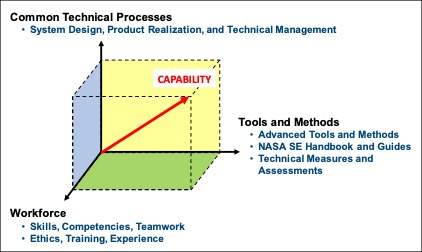
\includegraphics[width=0.7\linewidth]{figures/NPR7123.1DC1F4.jpg}
  \caption{NASA Systems Engineering Framework
  \cite{npr7123.1D}.}
  \label{fig:nasa_se_framework}
\end{figure}

This indicates a deeply embedded systems engineering culture that has explicit roles and job functions of systems engineers to support this framework. 
The framework’s strengths include clear accountability, comprehensive documentation and guidance, and alignment with agency-wide standards. 
The common technical processes mentioned here are defined at the Systems Engineering Engine \cite{npr7123.1D} that are comprise of 17 Technical Processes that are guided by the methods specified in the NASA SE Handbook \cite{nasa2016handbook} and other guiding documents. The 17 Technical Processes are:
\begin{enumerate}[noitemsep, topsep=0pt]
    \item Stakeholder Expectations Definition
    \item Technical Requirements Definition
    \item Logical Decomposition
    \item Design Solution Definition
    \item Product Implementation
    \item Product Integration
    \item Product Verification
    \item Product Validation
    \item Product Transition
    \item Technical Planning
    \item Requirement Management
    \item Interface Management
    \item Technical Risk Management
    \item Configuration Management
    \item Technical Data Management
    \item Technical Assessment
    \item Decision Analysis
\end{enumerate}
\subsection{OpenSE Framework}
\label{sub:opense}
OpenSE was developed within CERN’s Engineering Department as a systems-engineering approach explicitly tailored for scientific facilities \cite{cern2016opense,bonnal2018opense}. 
It was motivated by the recognition that research infrastructures differ fundamentally from aerospace or defense projects: they are collaborative, distributed, constrained by limited documentation cultures and evolving experimental designs, and must balance that with a focus on safety and reliability in the face of facilities with ionizing radiation. 
OpenSE aims to preserve the benefits of structured lifecycle management while reducing unnecessary process overhead.\\
The framework defines six phases (Initialize, Study, Design, Build, Commission, and Finalize) that parallel the ISO/IEC/IEEE 15288 lifecycle but with greater allowance for iteration and concurrency. \\
\begin{figure}[h]
  \centering
  
\includegraphics[width=0.9\linewidth]{figures/openSElifecycle.png}
  \caption{OpenSE Lifecycle
  \cite{cern2016opense}.}
  \label{fig:openSE_lifecycle}
\end{figure}

The framework notes in several places the inspiration from the NASA SE Handbook but that is more specialized and emphasizes tailorability from simple to more advanced approaches to the application of this framework. \cite{cern2016opense}
OpenSE emphasizes four guiding principles: openness, leanness, participation, modularity, and scalability.\cite{cern2016opense}
These principles shift the emphasis of governance that NASA takes through NPR 7123.1D \cite{npr7123.1D} and toward a minimal oversight expect safety kind of approach. The activities OpenSE describes are:
\begin{itemize}[noitemsep, topsep=0pt]
    \item Needs and Requirements 
    \item Integration
    \item Verification and Validation
    \item Solution Finding
    \item Safety Documentation
\end{itemize}
and are adapted from NASA's 17 Common Technical Processes.
\subsection{Minimal Frameworks}
\label{sub:minimal}
In contrast to structured or formal frameworks, many scientific collaborations, especially medium-scale research infrastructure, operate using minimal or ad hoc project management and subsequent systems engineering structures.
These approaches are characterized by limited lifecycle documentation, informal change control, if any, and reliance on experienced team leads for integration oversight rather than formal systems engineering artifacts. 
Most systems engineering practices are not highlighted as practices derived from this discipline but are largely viewed as compliance measure to meet facility requirements but are often considered after large portions of the research infrastructure are fabricated and assembled.
For this reason, there are not technical processes to discuss except derived characteristics which include Principle Investigator (PI)-driven design and facility requirements.
These will be referenced as Solution Finding, Integration, System Safety Verification, and ES\&H Documentation.
\subsection{Comparative Summary}
\label{sub:comparison}
Amongst the 3 approaches, NASA SE represents the most formalized and prescriptive model, emphasizing completeness, documentation, and mission assurance. 
OpenSE, while rooted in the same lifecycle principles, explicitly adapts these practices for research environments, reducing overhead while preserving modularity and openness. 
Minimal frameworks, by contrast, prioritize flexibility and speed at the cost of being formally verifiable and reproducible. 
The comparative characteristics of these frameworks, as synthesized from the literature, are summarized in Table \ref{tab:framework_comparison}.
\begin{table}[h]
\centering
\caption{A Summary of Common Elements Across Frameworks}
\label{tab:framework_comparison}
\begin{tblr}{
  colspec={|X[1.2,l]|X[1.5,l]|X[1.5,l]|X[1.5,l]|},
  hlines,
  row{1} = {font=\bfseries, halign=c},
  column{1} = {font=\bfseries},}
Characteristic & NASA SE & OpenSE & Minimal \\

Lifecycle Structure &
Sequential and gated &
Iterative and facility-driven &
Informal or project-defined \\

Problem Definition &
Stable once defined. 
Significant resources dedicated to requirements development. &
Functional requirements evolve while safety requirements are stable. 
Moderate resources dedicated to requirements development. &
Minimal time spent on requirements development. 
Reactive to safety and facility requirements. \\

Interface Management \& Integration &
Formalized.
Governed by ICDs. &
Structured but more flexible. 
Focuses on collaboration and shared understanding. &
Implicit and unstructured. 
Usually through verbal agreements or minimal documentation, as required by facility. \\

Verification \& Validation &
Formalized, following required V\&V plans. &
Formalized, following required V\&V plans. &
Informal or reactive to facility verification needs. 
Validation relies on in situ testing. \\

Flexibility &
Low to moderate. 
Suited for stable requirements. &
Moderate to high. 
Suited to evolving designs. &
High to very high. 
Suited for rapid development and changes. \\

Type/Domain &
First of a kind and high-stakes/aerospace, defense, missions. &
First or one of a kind, long-term, and iterative/research infrastructures, accelerators. &
First of a kind, demonstrators or prototypes/detectors, instruments, and bench-top R\&D labs. \\

Design \& Solution Finding &
Formalized and driven by agreed-upon requirements. 
Robust, multidisciplinary engineering studies. &
Somewhat formal with robust engineering. 
Driven by needs and requirements. 
Driven by physicists who act as both customer and engineer. &
Informal. 
Driven by PI needs. 
Driven by physicists who act as both customer and engineer. \\

Documentation \& Configuration Management &
Extensive, standardized artifacts. 
Robust engineering controls. &
Lean, scaled to project size. 
Engineering controls. &
Minimal, variable by team. 
Some or little engineering controls. \\
\end{tblr}
\end{table}

The characteristics were selected based on common activities or functions found across each framework.

\section{Advantages and Limitations of Systems Engineering}
\label{sect:pros&cons}

\paragraph{Advantages}
Many studies have been conducted over the last decade or more verifying the benefits of systems engineering. In an effort to not recreate many meta-analyses that already exist, this review will pull from well-known and established resources, primarily the Systems Engineering Book of Knowledge (SEBoK) \cite{sebok_economic_value}. In the review of the economic benefits of systems engineering in SEBoK, a study highlighting the criticality of systems engineering for NASA missions is discuessed. Figure \ref{fig:se_investments} illustrates the relationship between the percentage of project resources devoted to systems engineering and the percentage of project cost overrun.\cite{sebok_economic_value} \\

\begin{figure}[h]
  \centering
  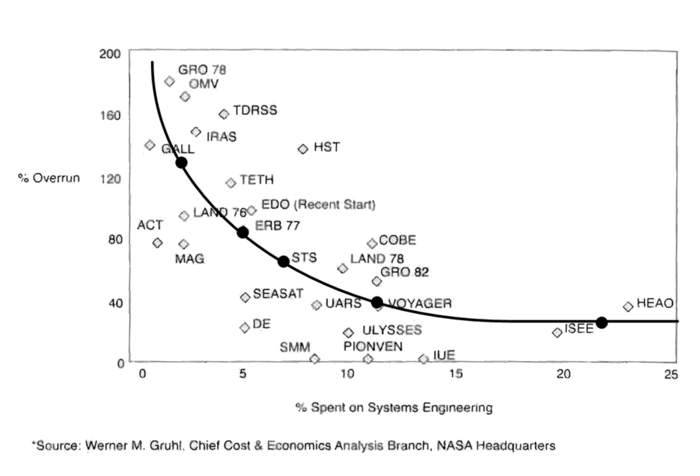
\includegraphics[width=0.7\linewidth]{figures/700px-NASA_Image_Part_1.png}
  \caption{Relation of SE Investments to NASA Program Cost Overruns (Stutzke 2005)
  \cite{sebok_economic_value}.}
  \label{fig:se_investments}
\end{figure}

Data from NASA programs show that projects investing less than 5\% in systems engineering experienced overruns exceeding 150\%, while those allocating greater than 15\% maintained very low overruns. 
This trend demonstrates that robust systems engineering practices reduce technical and programmatic with some enhanced cost and schedule predictability. 
According to this study, even a modest increase in systems engineering investment yields significant benefits in project controls success. 
The gap here is understanding the impacts on this correlation if system performance or mission success were factored in.\\
It is evident that there needs to have a balance struck on time and resources spent on systems engineering and complexity of a system or project.\cite{sebok_economic_value} 
The relationship between the percentage of project time devoted to initial architectural design and risk resolution versus the total schedule impact, including rework, is illustrated in Figure \ref{fig:enoughSE}. 
 
\begin{figure}[h]
  \centering
  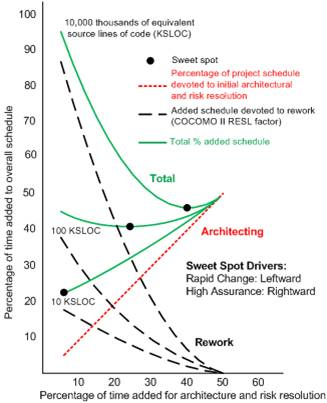
\includegraphics[width=0.7\linewidth]{figures/P1_EconValueSE_RiskBalancedfig2_BB.jpg}
  \caption{Risk-Balanced “How Much SE Is Enough” (Boehm, Valerdi, and Honour 2008)
  \cite{sebok_economic_value}.}
  \label{fig:enoughSE}
\end{figure}

There is clear optimum or "sweet spot" where fairly moderate early investment in architecture and risk management minimizes overall schedule growth. 
Projects that spend too little time in these early phases face substantial rework later, while excessive early analysis can also extend schedules unnecessarily. Physicist and engineers alike can fall prey to "analysis paralysis."
Effective systems engineering finds the balance, ensuring that sufficient effort is applied early to reduce downstream uncertainty and rework, ultimately improving schedule efficiency and project assurance.
Most systems engineering frameworks, if structured well, provide precisely that: tailorability in application (even the more rigid frameworks). 
And that is at the heart of what question being asked here - what is "enough" for medium-scale research infrastructure projects and is OpenSE a viable tailored framework? 
Bonnal et al.\cite{bonnal2018opense} describes OpenSE as “particularly suited to particle-accelerator studies and development projects,” noting its flexibility for projects with shared governance and partial reuse of existing infrastructure (i.e., facility infrastructure from previous experiments).

\paragraph{Limitations}
Multiple analyses have noted that the strengths of rigid systems engineering can impose significant administrative overhead and reduce flexibility when applied to small or exploratory projects \cite{r&dSE}. 
The rigor of NASA SE can thus exceed the practical capacity of medium-scale research infrastructure projects or research-driven teams, particularly those operating with evolving scientific objectives or limited dedicated engineering staff.
Kaeske et al. \cite{Kaeske_Wagner_Albers_Russenschuck_2024} discuss the usefulness of the framework but highlight the needs for more prescriptive methodology and tool support to bridge the gap between intentional generalizations and practical guidance.
Honoré-Livermore et al. \cite{academicsPerceptionSE} and Hodges and Granados \cite{r&dSEbridge} highlight that early-stage R\&D projects often view traditional systems engineering as incompatible with their culture of rapid iteration and discovery. 
Instead, these early-stage R\&D projects apply systems engineering principles selectively, focusing on design and documentation only when required for compliance with a funding organization or the facility hosting the system.

\paragraph{Identified Gaps and Solutions for R\&D}
There is this term called the “Valley of Death” that typically arises at Technology Readiness Levels (TRLs) 5 and 6, where responsibility transitions from early-stage research to full-scale development. 
This phase often becomes a point of friction between exploratory R\&D engineers and those focused on later development at TRLs 7 and higher.\cite{r&dSE} 
Many efforts fail to progress beyond this stage due to insufficient funding, performance gaps, or inadequate mechanisms to bridge research outputs with operational capability. 
Additional causes include unclear research objectives (requirements), poorly managed risks, weak coordination between transitioning organizations (knowledge and interface management), and ineffective application of processes (training and methods). 
Misaligned performance measures, leadership conflicts, and entrenched cultural factors can further exacerbate the issue. 
Ultimately, the findings keep coming back to selecting and implementing the right framework for the project at hand.

\section{Research Infrastructure Project Metrics}
\label{sect:metrics}
So how do we choose the right framework for the project at hand?
The first step might be to characterize what goals the project is trying to achieve and how it intends to measure its success at getting to those goals.
Limited studies or interviews exist to quantify how research experiments, beyond individual experiments of physics runs, quantify success, highlighted by Stotz and Drews.\cite{experimentMetrics} The metrics they did discover after their study were grouped into six categories: 
\begin{enumerate}
    \item \textbf{Volume:} scale and reach of experimentation
    \item \textbf{Outcome-Based:} results and impact of experimentation
    \item \textbf{Quality:} rigor and reliability of experimentation
    \item \textbf{Engagement and Adoption:} how widely experimentation practices are embraced
    \item \textbf{Process Efficiency:} duration from experiment setup to actionable results
    \item \textbf{Strategic Alignment:} impact on broader organizational goals
\end{enumerate}

These categories can easily be mapped back to typical project metrics that give a foundation for the simulation-based study. Volume translates to uptime, outcome-based translates to earned value, quality translates system performance and data integrity, engagement and adoption translates to customer satisfaction, process efficiency translates to schedule, and strategic alignment translates to stakeholder satisfaction.\\
More specific mapping to the simulation will be discussed in the \ref{chapter:methods}.
\section{Gaps in Simulation-Based Research}
\label{sect:simulations}
To date, this project's efforts have not found any studies or research using simulation-based methods to compare systems engineering frameworks impact to performance in the context of scientific research infrastructure projects. 
Further efforts should be made to find alignment between research that exists in similar domains to inform the future work performed.
\clearpage
\chapter{Methods}
\label{chapter:methods}
\paragraph{Preamble and Caveat} First and foremost, it is important to note that all parameter distributions and coefficients are illustrative and chosen to reflect qualitative differences among frameworks rather than measured quantities.
Values are based on engineering judgment and prior experience in research infrastructure projects, specifically COHERENT.
The model is intended to demonstrate structure and possible sensitivity, not to forecast actual science yield.
A recommended next step is to create dynamics loops that better represent behaviors, replace these assumed distributions with data from project lessons learned or
published later applicable systems engineering effectiveness studies.\\

A Monte Carlo simulation approach was implemented to estimate the expected distribution of science data loss across three systems engineering (SE) frameworks: NASA SE, OpenSE, and a Minimal. 
The simulation was performed in Python using NumPy, Matplotlib, and Pandas libraries for numerical computation, visualization, and data aggregation, respectively.

A total of $N = 100{,}000$ iterations were executed per framework to ensure statistical stability in the resulting distributions. 
Each iteration generated a artificial realization of eight independent parameters representing major project performance drivers, summarized in Table \ref{tab:variables}. 
\begin{table}[htbp]
    \centering
    \caption{Simulation Variables and Descriptions}
    \label{tab:variables}
    \begin{tabular}{llp{8cm}}
        \toprule
        \textbf{Variable} & \textbf{Symbol} & \textbf{Description and Rationale} \\
        \midrule
        Duration Overrun & $D$ & Fractional increase beyond baseline schedule. Reflects planning discipline and lifecycle control. \\
        Rework Fraction & $R$ & Portion of effort required for correcting or revisiting previous work. Indicates quality of initial execution and requirement clarity. \\
        Integration Readiness & $IRL$ & Scaled to [0, 1], where 1 represents fully integrated, interface-mature components. IRLs are one a 1-9 scale that mirrors TRLs.\cite{gao2020tra} Captures coordination and pre-integration maturity. \\
        Maintenance Downtime & $T_m$ & Expected fractional time lost due to system unavailability. Reflects robustness, results of performing FMEAs, and having support engineering. \\
        Design Compromise & $P$ & Degree of functional or performance trade-offs made during development. Includes scope reduction and underperformance. \\
        Budget Reallocation & $B_1$ & Portion of budget diverted due to unforeseen work (e.g., rework, emergent tasks). \\
        Inefficiencies and overburden documentation & $I$ & Fractional loss due to admin burden. Assumption based on procedural inefficiency estimates, slow decision-making.\\
        Measurement Degradation & $Q$ & Captures the loss of data quality due to instrumentation or procedural faults. Affects science yield directly. \\
        \bottomrule
    \end{tabular}
\end{table}


These include duration overrun ($D$), rework fraction ($R$), integration readiness level ($IRL$), maintenance downtime ($T_m$), design compromise severity ($P$), budget reallocation due to rework ($B_1$), inefficiencies and overburden ($I$), and measurement quality degradation ($Q$). 
Each parameter was expressed as a normalized fraction of impact (0–1) or readiness (for $IRL$), allowing combination into a unified performance index.
These parameters are an initial derivation from the literature review.\\
For each framework, the parameters were sampled from either bounded normal or triangular distributions. 
These distribution shapes were chosen based on the level of uncertainty and skew expected from the framework’s project management characteristics and how well studied the implementation of these approaches are. 
For example, NASA SE emphasizes documentation rigor, leading to slower progress but lower variance in integration readiness, whereas Minimal exhibits greater uncertainty due to weak control and lack of formal processes. The varying standard deviations were informed by how characterized or studied these impacts are, in general, as well.\\
Each framework’s parameterization is summarized below:
\begin{itemize}
    \item \textbf{NASA SE:} conservative lifecycle durations, high effort, and strong reliability and safety focus. 
    \item \textbf{OpenSE:} iterative and lean processes with moderate formality and focus on safety.
    \item \textbf{Minimal:} loosely coordinated workflows with higher performance, schedule, and cost volatility, but greater flexibility.
\end{itemize}

Initial simplicity was the goal and thus the overall science data loss fraction ($L$) was computed as the normalized mean of the eight contributing parameters:
\begin{equation}
    L = \frac{D + R + (1 - IRL) + T_m + P + B_1 + I + Q}{8},
\end{equation}
where $L$ represents the effective fraction of total potential science yield lost due to engineering inefficiencies or integration challenges. All values were constrained within the $[0, 1]$ range.\\
A summary of simulation statistics was computed for each framework, including mean ($\mu_L$), standard deviation ($\sigma_L$), 5th and 95th percentiles, and the probability of exceeding a 10\% data loss threshold, $P(L > 0.1)$, which serves as a risk indicator for unacceptable performance degradation.\\

\vspace{1em}
\noindent The full Python script used for this analysis is included in the GitHub repository \hyperref[https://github.com/hannahmclaurin/syse695-masters-planB]{\textbf{syse695-masters-planB}} where this report is also maintained.

\clearpage
\chapter{Results}
\label{chapter:results}

Figure \ref{fig:initial} shows the resulting probability density distributions for the simulated science data loss across the three frameworks. \\
\begin{figure}[h!]
  \centering
  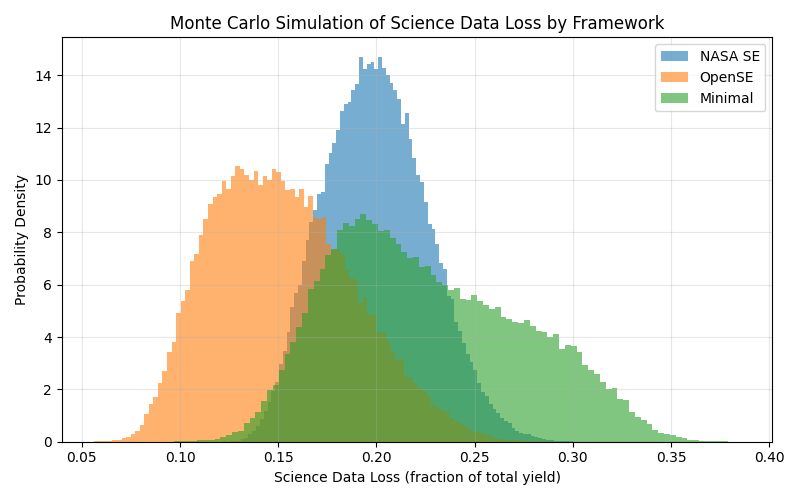
\includegraphics[width=0.9\linewidth]{figures/initial_distribution.png}
  \caption{Initial Scientific Yield Loss Monte Carlo Distribution}
  \label{fig:initial}
\end{figure}

NASA SE displays a narrow, low-loss distribution consistent with highly structured engineering control. OpenSE exhibits a broader spread with a slightly higher mean loss, reflecting its iterative and flexible implementation approach. The Minimal workflow demonstrates the widest spread and highest probability of significant loss, indicative of unmanaged variability and weak lifecycle controls.\\

The summary statistics for all three frameworks are shown in Table \ref{tab:results_summary}. \\
\begin{table}[htbp]
  \centering
  \caption{Summary of Statistics}
  \label{tab:results_summary}
  \begin{tabular}{lccc}
    \toprule
    \textbf{Metric} & \textbf{NASA SE} & \textbf{OpenSE} & \textbf{Minimal} \\
    \midrule
    Mean $L$             & 0.200 & 0.152 & 0.226 \\
    Std.\ $L$            & 0.026 & 0.036 & 0.048 \\
    5th Percentile       & 0.158 & 0.100 & 0.157 \\
    95th Percentile      & 0.245 & 0.216 & 0.312 \\
    $P(L > 10\%)$        & 1.000 & 0.950 & 1.000 \\
    \bottomrule
  \end{tabular}
\end{table}

The probability of exceeding 10\% science data loss, $P(L>0.1)$, was lowest for NASA SE and highest for the Minimal case, with OpenSE positioned in between—suggesting that moderate formalism combined with agility may reduce risk without incurring excessive process overhead.

\clearpage
\chapter{Discussion}
\label{chap:discussion}
%THIS IS PRELIMINARY AND MAY CHANGE%
The results of the Monte Carlo simulation provide insight into the expected science data loss across three systems engineering frameworks: NASA SE, OpenSE, and a Minimal framework.\\
Overall, the OpenSE framework demonstrates the lowest mean simulated science data loss ($\mu = 0.152$), followed by NASA SE ($\mu = 0.200$), with the Minimal framework performing worst ($\mu = 0.226$). While NASA SE is traditionally associated with high procedural rigor and reliability, its high burden of procedural overhead may offset its gains in schedules where quicker turn around and flexibility are often required for exploratory research projects.\\
Despite OpenSE’s looser structure, it benefits from lower rework levels and a balance between flexibility and formality, which likely contributes to its lower science loss. The broader variance (Std.\ $L$ = 0.036) suggests more sensitivity to project conditions but still maintains "acceptable" performance.\\
In contrast, the minimal framework shows both higher mean loss and greater variance (Std.\ $L$ = 0.048), confirming expectations about the risk of adopting ad hoc approaches for medium-scale projects where complexity is increasing. 
The 95th percentile loss for Minimal (0.312) indicates a long tail of worst-case scenarios, reflecting a possible increased risk in scientific output degradation.\\
The probability of exceeding a 10\% science loss threshold is nearly certain for all frameworks ($P(L > 10\%)$ > 0.950), but OpenSE is the only framework that shows any meaningful chance of staying below this threshold, indicating potential suitability in environments that demand both flexibility and scientific reliability.\\
These findings partially reinforce a hypothesis that neither extreme formality nor minimal structure is optimal for medium-scale research infrastructure.
Frameworks like OpenSE, designed for scientific environments, may offer a better trade-off between structure and agility.
\clearpage
\backmatter
\clearpage
\bibliographystyle{unsrt}
\bibliography{references}
\clearpage
\appendix
\clearpage
\end{document}